\documentclass[../relazione.tex]{subfiles}

\begin{document}
\section{Progettazione}
	\subsection{XHTML}
	\begin{itemize}
		\item Logo come background tramite IMAGE REPLACEMENT cosicchè possa costituire informazione per il motore di ricerca (Best practice)
		\item Sostituita immagine del bottone di navigazione con il carattere come su \url{http://www.w3schools.com}
		\item il path svolge sia funzione di breadcrumb che di titolo della pagina, per siti che hanno un solo livello profondità non serve breadcrumb
		\item Termini caratteristici usato <strong> per SEO
	\end{itemize}
	\subsection{CSS}
	\begin{itemize}
		\item 
	\end{itemize}
	\subsection{Perl/CGI}
	\begin{itemize}
		\item 
	\end{itemize}
	\subsection{Javascript}
	\begin{itemize}
		\item Nav inizialmente visibile, così se non c'è JS ho degradazione elegante. Se JS funziona, allora viene nascosto e rimane accessibile dall'apposito bottone
		\item è presente il controllo dei dati inseriti nei campi nelle form di login, aggiunta e modifica
	\end{itemize}
	\subsection{XML e XMLSchema}
	\begin{itemize}
		\item 
	\end{itemize}
	\subsection{Mobile}
	riportare motivi per cui è stata implementata anche la versione mobile
	\begin{itemize}
		\item menù può essere accessibile da mobile
		\item usato la "hamburger icon", ritenuta adeguata perché ormai consuetudine per gli utenti associare essa al menu del sito
		\item abbiamo pensato che fosse comodo per l'utente poter aprire e chiudere il menu del sito (nav), per agevolare la visita del sito, per rendere più piacevole l'esperienza: per far ciò è stata utilizzata una funzione Javascript che mostra e nasconde il nav attraverso l'icona hamburger
		\item il sito è stato testato sui seguenti browser mobile: Google Chrome, Safari
	\end{itemize}
	\begin{figure}[H]
		\centering
		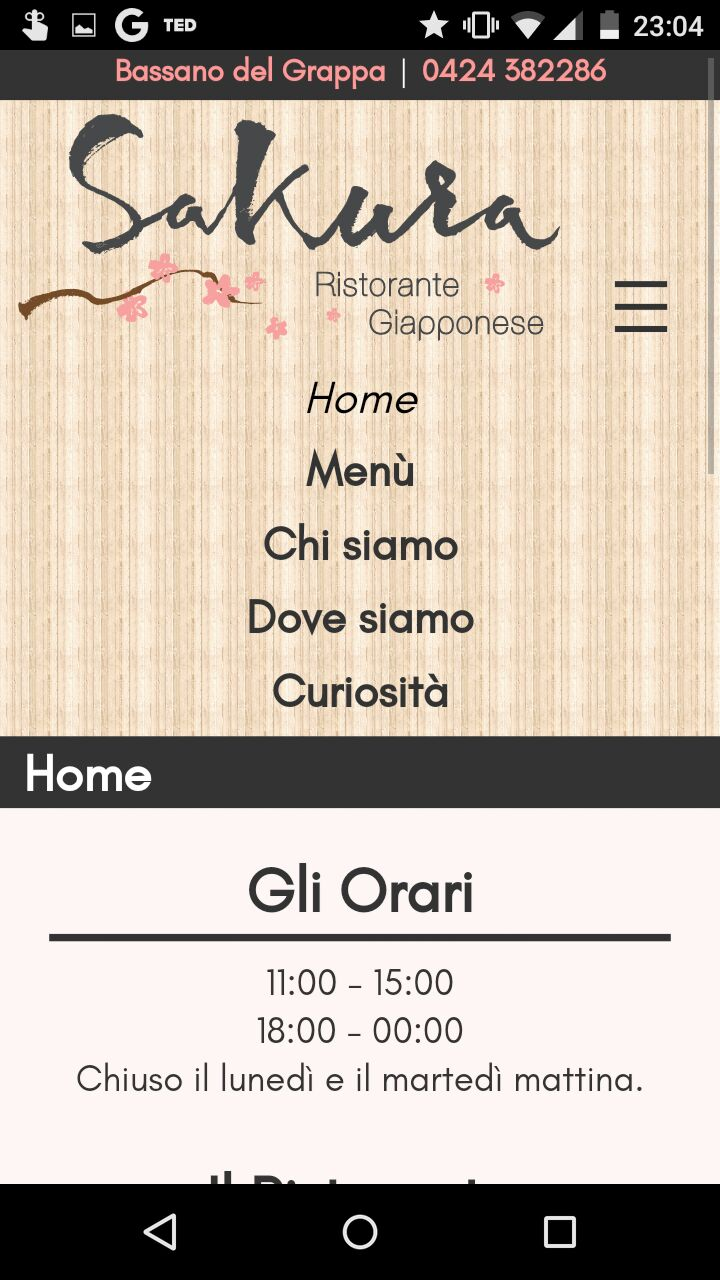
\includegraphics[scale=0.2]{images/mobile2}
		\caption{Esempio di pagina vista da dispositivo mobile}
		\label{fig:Esempio di pagina vista da dispositivo mobile}
	\end{figure}
\end{document}